\documentclass[
    notheorems,
    11pt,
    compress,
    aspectratio=169
]{beamer}

\mode<presentation>{
    \usetheme{Madrid}
    \usecolortheme{orchid}
    \usefonttheme[onlymath]{serif}
    \setbeamertemplate{blocks}[rounded][shadow=true]
    \setbeamertemplate{navigation symbols}{}
    \setbeamertemplate{enumerate items}[square]
}

\usepackage{config}

\graphicspath{{./figures/}}
\bibliography{bibliography.bib}

% -----

\title[Conosciamo gli algoritmi e i linguaggi]{Dal problema al programma: le basi della programmazione}
\subtitle{Conosciamo gli algoritmi e i linguaggi}
\author{prof. Leonardo Essam Dei Rossi}
\institute[]{ITT "M. Buonarroti" - Trento (TN)}
\date[A.S. 2025/2026]{Anno scolastico 2025/2026}

% -----

\begin{document}

\setlength{\baselineskip}{15pt}

\begin{frame}
\titlepage
\end{frame}

\begin{frame}
    \frametitle{Indice}

    \tableofcontents
\end{frame}

% -----

\section{I problemi e la loro soluzione}

\begin{frame}{I problemi e la loro soluzione (1)}
    In ogni ambito e settore, dalle scienze alla economia, dalla biologia alla tecnologia, dallo sport alla vita quotidiana, ciascuno di noi deve giornalmente affrontare dei \textbf{problemi}, eseguire dei \textbf{compiti} e prendere delle \textbf{decisioni}.

    \pause
    \vfill
    
    \begin{block}{Esempio}
        Ci capita regolarmente di “ripartire il costo” di una pizzata tra amici, di scegliere un film o un regalo da fare a un amico per un compleanno, di dover organizzare la serata oppure tagliare l’erba in giardino o mettere in ordine i nostri libri e gli appunti scolastici.
    \end{block}
\end{frame}

\begin{frame}{I problemi e la loro soluzione (2)}
    Siamo in grado di risolvere la maggior parte dei \textbf{problemi} che affrontiamo perché o sono \textbf{semplici} oppure perché li abbiamo già “fatti almeno una volta” in passato, e quindi ci basiamo sulla nostra esperienza o sulla consulenza di qualche amico.

    \pause
    \vfill

    Per altri \textbf{problemi}, invece, la ricerca della \textbf{soluzione} a volte ci risulta difficile, se non impossibile, soprattutto se ci mancano delle conoscenze o delle informazioni (\textit{dati}) oppure se la difficoltà intrinseca della situazione lo rende un enigma.
\end{frame}

\begin{frame}{I problemi e la loro soluzione (3)}
    \begin{block}{Definizione: problema}
        Il matematico e l’informatico identificano con la parola \textbf{problema} una questione (o quesito) che deve essere risolta, della quale viene data una situazione con dei \textbf{dati} iniziali noti e un obiettivo, che consiste nella soluzione desiderata.

        \vspace{0.25cm}
        
        La \textbf{soluzione} di un problema consiste nella deinizione della procedura ovvero le operazioni che devono essere eseguite per raggiungere lo scopo desiderato.
    \end{block}
\end{frame}

\begin{frame}{I problemi e la loro soluzione (4)}
    \textbf{I problemi non sono tutti uguali tra loro, né per tipologia, né per complessità.}
    
    \pause
    
    Per individuare la \textbf{soluzione} poterebbe essere necessario cercare di comprendere meglio il problema, cioè effettuare un’\textbf{analisi} approfondita della situazione e, nei casi più complessi, individuare una \textbf{strategia risolutiva}.

    \pause
    \vfill

    \begin{block}{Definizione: strategia risolutiva}
        Con strategia risolutiva si intende la modalità con la quale si risolve il problema, cioè l’idea con la quale il programmatore sfruttando l’esperienza, l’intuito, fantasia e, perché no, l’intelligenza affronta il processo creativo relativo e trova la “chiave di soluzione” del problema.
    \end{block}
\end{frame}

% -----

\subsection{Un esempio "classico"}

\begin{frame}{Un esempio "classico" (1)}
    Per meglio comprendere cosa si intende per \textbf{soluzione} e per \textbf{strategia risolutiva} descriviamo un famoso problema, noto col nome di: \textit{il contadino, il lupo, la capra e il cavolo}.

    \pause
    \vspace{0.5cm}

    Sulla riva di un fiume ci sono un contadino, un lupo, una capra e un cavolo che devono attraversare un fiume con una piccola barca: su di essa è possibile portare solo due “cose” alla volta.

    \pause
    \vspace{0.5cm}

    Come può il contadino attraversare indenne il fiume salvando “capra e cavoli” sapendo che se vengono lasciati da soli il lupo con la capra, oppure la capra con il cavolo, i primi divorano i secondi?
\end{frame}

\begin{frame}{Un esempio "classico" (2)}
    La situazione che ci viene proposta è sufficientemente chiara e definita che non necessita ulteriori richieste di delucidazioni.

    \vspace{0.25cm}

    Sinteticamente analizziamo la nostra situazione e riformuliamo il problema:

    \begin{itemize}
        \item Abbiamo un obiettivo (goal), che è quello di traghettare un contadino e le “tre cose” che ha con se tra due rive di un fiume;

        \item Abbiamo un limite di cose che possiamo portare sulla barca (vincolo): due alla volta;

        \item Dobbiamo stare attenti a cosa lasciamo incustodito sulla riva mentre il contadino sta remando (vincolo) in quanto:

        \begin{itemize}
            \item Se rimane il lupo con la capra... quest’ultima viene mangiata;

            \item Se rimane la capra con il cavolo... quest’ultimo viene mangiato.
        \end{itemize}
    \end{itemize}
\end{frame}

\begin{frame}{Un esempio "classico" (3)}
    Il nostro compito è quello di trovare la soluzione di questo problema, che consiste nel “suggerire” al contadino cosa deve fare, cioè che tipo di operazione deve eseguire (chi portare sulla barca) e come deve farla, cioè in che ordine.

    \pause
    \vfill

    \textbf{In altre parole dobbiamo dargli le “istruzioni risolutive” indicandogli la sequenza esatta.}

    \pause
    \vfill

    La strategia risolutiva in questo caso consiste nella individuazione della corretta sequenza delle operazioni che il nostro contadino-traghettatore deve effettuare per effettuare con esito positivo la traversata.
\end{frame}

\begin{frame}{Un esempio "classico" (4)}
    Come nel caso appena descritto capita spesso di dover indicare ad altri la soluzione del problema, cioè descrivere la procedura risolutiva, e questo deve essere fatto in modo tale che chi la deve eseguire la possa comprendere senza possibilità errore.

    \pause
    \vspace{0.5cm}

    La soluzione viene descritta solitamente indicando l’insieme delle operazioni (passi) che devono essere effettuati riportandoli nell’ordine in cui devono essere eseguiti (sequenza di operazioni).

    \pause
    \vspace{0.5cm}

    \textbf{È di fondamentale importanza che l’esecutore sia in grado di comprendere le istruzioni che permettono di risolvere il problema e, inoltre, sia un grado di eseguirle.}
\end{frame}

% -----

\subsection{Esercizio}

\begin{frame}{Esercizio}
    Un agricoltore deve diluire un sacco di fertilizzante in 20 litri d’acqua, ma ha a disposizione un annafi atoio con capacità 25 litri contenente 16 litri d’acqua e due contenitori rispettivamente da 5 e 3 litri.

    \vspace{0.25cm}

    \textbf{Come può operare l’agricoltore?} \textit{Descrivi a parole le sequenza delle operazioni necessarie a ottenere esattamente 20 litri nell’annafiatoio.}

    \vspace{1cm}

    \begin{columns}
        \column{0.3\textwidth}
        
        \begin{block}{}
            \centering
            Affrontare\\un problema
        \end{block}
        
        \column{0.3\textwidth}
        
        \begin{block}{}
            \centering
            Ricercare la\\strategia risolutiva
        \end{block}

        \column{0.3\textwidth}
        
        \begin{block}{}
            \centering
            Scomporre in\\istruzioni/passi
        \end{block}
    \end{columns}
\end{frame}

% -----

\section{Il concetto di "algoritmo"}

\begin{frame}[fragile]
    \frametitle{Il concetto di "algoritmo" (1)}
    
    Abbiamo visto che partendo dal problema per arrivare alla soluzione è necessario analizzare dettagliatamente la situazione e individuare la strategia risolutiva, cioè “trovare” l’idea che risolve la situazione.

    \pause
    \vfill

    \begin{figure}
        \centering
        \begin{tikzpicture}[
            box/.style={
                draw=blue!80!black,
                fill=blue!10,
                rectangle,
                rounded corners,
                minimum width=2.75cm,
                minimum height=1cm,
                align=center,
                font=\sffamily\footnotesize
            },
            arrow/.style={
                ->,
                thick,
                >=stealth
            }
        ]

            \node[box] (step1) {\textbf{Il problema}};
            \pause
            
            \node[box, right=0.5cm of step1] (step2) {\textbf{L'analisi}};
            \draw[arrow] (step1) -- (step2);
            \pause
            
            \node[box, right=0.5cm of step2] (step3) {\textbf{L'idea}\\La strategia};
            \draw[arrow] (step2) -- (step3);
            \pause
        
            \node[box, right=0.5cm of step3] (step4) {\textbf{La soluzione}\\L'algoritmo};
            \draw[arrow] (step3) -- (step4);
        \end{tikzpicture}    
    
        \caption{Dal problema all'algoritmo}
        \label{fig:fig21}
    \end{figure}

    {\usebeamercolor[fg]{structure}Figura \ref{fig:fig21}:} \cite[p. 323]{ISBN_8820378434}
\end{frame}

\begin{frame}{Il concetto di "algoritmo" (2)}
    Quando la strategia risolutiva è stata definita, quindi quando si è “scoperto” il criterio risolutivo del problema, bisogna “scrivere” le singole istruzioni che l’esecutore deve compiere, in sequenza, una dopo l’altra.

    \pause
    \vspace{0.5cm}

    \textbf{L’insieme delle operazioni che permettono di risolvere un problema prende il nome di algoritmo.}
\end{frame}

\begin{frame}{Il concetto di "algoritmo" (3)}
    \begin{columns}
        \column{0.4\textwidth}

        \begin{figure}[h]
            \centering
            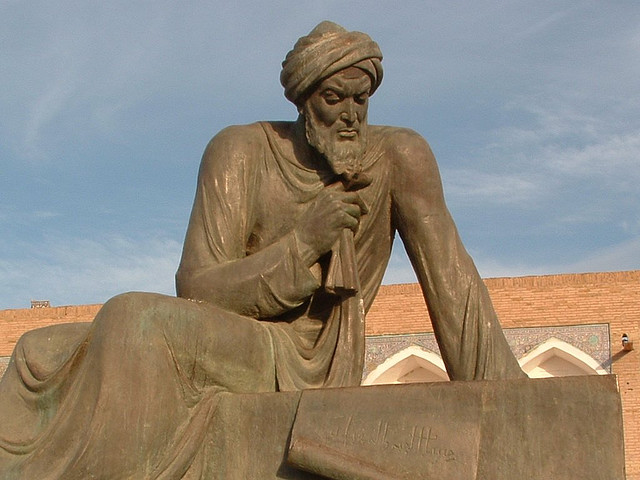
\includegraphics[width=0.8\textwidth]{figures/fig02-alkhwarizmi.jpg}
        \end{figure}

        \column{0.6\textwidth}

        Il termine algoritmo è una “deformazione” del nome del matematico arabo al-Khwarizmi, vissuto nel IX secolo d.C., ritenuto l’ideatore del procedimento che consente di effettuare il calcolo della moltiplicazione tra due numeri mediante la disposizione a cifre incolonnate (che è quella che usiamo ancora oggi).
    \end{columns}
\end{frame}

\begin{frame}{Il concetto di "algoritmo" (4)}
    \begin{block}{}
        Quindi l’algoritmo non è altro che una sequenza ordinata di passi semplici che hanno lo scopo di portare a termine un compito a volte complesso.
    \end{block}

    \vspace{0.5cm}

    Anche la ricetta per la preparazione della pizza o di un qualunque piatto è a tutti gli effetti un algoritmo, dato che descrive a partire dagli ingredienti le operazioni che, in sequenza, devono essere eseguite passo passo, per ottenere come risultato il piatto desiderato.
\end{frame}

% -----

\section{Il linguaggio che descrive l’algoritmo}

\begin{frame}{Il linguaggio che descrive l’algoritmo (1)}
    L’algoritmo deve essere descritto in modo chiaro, in un linguaggio che sia comprensibile per il suo esecutore, che non necessariamente deve essere un umano, ma può anche essere una macchina (un calcolatore elettronico oppure un automa elettromeccanico).

    \pause
    \vspace{0.25cm}

    Se per un essere umano è sufficiente descrivere le istruzioni “a parole”, cioè utilizzando un linguaggio naturale (cioè la lingua che parliamo) oppure una forma grafica, ad esempio utilizzando i diagrammi a blocchi (flow chart) che vedremo nella prossima lezione, se l’esecutore è una macchina è necessario individuare una “forma” particolare che ci permette di comunicare con essa.
\end{frame}

\begin{frame}[fragile]
    \frametitle{Il linguaggio che descrive l’algoritmo (2)}
    
    \textbf{La descrizione di un algoritmo in linguaggio naturale prende il nome di pseudocodifica.}

    \vspace{0.25cm}
    \hrule
    \vspace{0.25cm}

    Scriviamo la pseudocodifica dell’algoritmo che ci permette di inviare un messaggio col cellulare:

    \begin{block}{}
        \begin{enumerate}
            \item Accendi il telefono;
            \pause
            \item Seleziona la app opportuna tra quelle presenti nel tuo telefono;
            \pause
            \item Se il numero del destinatario è presente nella tua rubrica:
            \begin{enumerate}
                \item Seleziona il numero digitando il nome o facendo scorrere l’elenco;
                \item Altrimenti digita il numero sulla tastiera numerica.
            \end{enumerate}
            \pause
            \item Compila il messaggio da inviare;
            \pause
            \item Clicca sull’icona \verb|<invio>|
        \end{enumerate}
    \end{block}
\end{frame}

\begin{frame}{Il linguaggio che descrive l'algoritmo (3)}
    \begin{block}{}
        Questa codifica non è univoca: possiamo descrivere l’algoritmo sia con parole diverse che con sequenze diverse di istruzioni, pur non compromettendone la correttezza.

        \vspace{0.25cm}
        
        Ad esempio potremmo avere casi più articolati in cui nella app è già presente una conversazione attiva e quindi la scelta delle opzioni diviene più articolata con possibili alternative di scelta e, quindi, un algoritmo più “elaborato”.
    \end{block}

    \vfill

    \textbf{L’algoritmo deve essere il più possibile generale, cioè contemplare tutte le possibili situazioni e non un caso specifico.}
\end{frame}

% -----

\subsection{Esercizio}

\begin{frame}{Esercizio}
    \begin{columns}
        \column{0.4\textwidth}

        \begin{figure}[h]
            \centering
            
\includegraphics[width=0.65\textwidth]{figures/fig03-pizzamargherita.jpg}
        \end{figure}

        \column{0.6\textwidth}

        Scrivi la procedura per preparare e cuocere una pizza margherita partendo dai suoi componenti e indicando dettagliatamente ogni singola operazione, una per riga.
    \end{columns}

    \vspace{0.5cm}

    \begin{columns}
        \column{0.45\textwidth}
        
        \begin{block}{}
            \centering
            Definizione dell’algoritmo
        \end{block}
        
        \column{0.45\textwidth}
        
        \begin{block}{}
            \centering
            Codifica in pseudocodice
        \end{block}
    \end{columns}
\end{frame}

\begin{frame}{Il linguaggio che descrive l'algoritmo (4)}
    \textbf{Né la descrizione in linguaggio naturale né i diagrammi a blocchi sono adatti per scrivere programmi che devono essere eseguiti dagli elaboratori elettronici.}

    \pause
    \vspace{0.25cm}

    Tra gli elaboratori elettronici includiamo tutti i dispositivi che “hanno al loro interno” un sistema programmabile, cioè un microprocessore: rientrano tra questi il PC, lo smartphone, la console per videogiochi, ma anche la lavatrice, l’ascensore, l’automobile, la bilancia, ecc.
\end{frame}

\begin{frame}{Il linguaggio che descrive l'algoritmo (5)}
    Sappiamo che il microprocessore è un dispositivo che è in grado di comprendere istruzioni codificate in binario: quindi, nella memoria di un dispositivo in grado di eseguire un programma in modo autonomo, deve essere presente il codice binario (detto programma binario o codice eseguibile in linguaggio macchina).

    \pause
    \vspace{0.25cm}

    \textbf{Gli esseri umani, però, faticosamente riescono a scrivere codice binario!}
\end{frame}

\begin{frame}{Il linguaggio che descrive l'algoritmo (6)}
    Se da una parte la pseudocodifica risulta inadatta alla scrittura del programma perché è troppo vicino all’uomo (linguaggio naturale), dall’altra anche il codice binario si rivela inadeguato perché è troppo vicino alla macchina (basso livello): è necessario individuare una soluzione intermedia e a tal fine sono stati “inventati” i linguaggi di programmazione.

    \pause
    \vspace{0.25cm}

    \begin{block}{Definizione: programmatore}
        Con il termine programmatore si indica una persona che scrive programmi, cioè algoritmi codificati in un linguaggio adeguato (linguaggio di programmazione) afi nché possa essere “compreso” da una macchina.
    \end{block}
\end{frame}

\begin{frame}{Il linguaggio che descrive l'algoritmo (7)}
    Possiamo sintetizzare in due tappe fondamentali la “nascita della programmazione” degli elaboratori:

    \vspace{0.25cm}

    \begin{block}{Nel "paleolitico"}
        Nella \textit{"preistoria"} dell’informatica i programmatori “programmavano in binario”, o meglio, producevano codice binario. Il processo era lungo in quanto si partiva dal problema, quindi si scriveva l’algoritmo in linguaggio naturale, poi lo si riscriveva riducendo la tipologia di istruzioni e avvicinandosi sempre di più alla descrizione con le sole operazioni che la CPU era in grado di eseguire e, come ultimo passaggio, lo si traduceva in zeri e uno!
    \end{block}
\end{frame}

\begin{frame}{Il linguaggio che descrive l'algoritmo (8)}
    \begin{block}{Nel "neolitico"}
        Successivamente per ottenere questa conversione si è ricorsi a un apposito programma, chiamato compilatore (o traduttore), in grado di trasformare in codice binario un programma scritto utilizzando un linguaggio vicino al programmatore, cioè ad alto livello, ma composto da poche parole (parole chiave o riservate) scritte con una sintassi molto rigorosa, proprio perché doveva essere “capito” da una “macchina stupida”: sono nati così, attorno agli anni Cinquanta, i primi linguaggi di programmazione ad alto livello.
    \end{block}
\end{frame}

% -----

\subsection{La programmazione oggi}

\begin{frame}{La programmazione oggi (1)}
    \begin{block}{}
        Esistono oggi veramente tanti linguaggi di programmazione (oltre 2500 e sono in continuo aumento!): la proliferazione di linguaggi di programmazione è giustiicata da oggettive necessità di specializzazione o da innovazione tecnologica che richiedono nuove tecniche e istruzioni sempre più soisticate per rendere più agevole lo sviluppo di applicazioni complesse.
    \end{block}

    \pause
    \vspace{0.5cm}

    Tra tutti i linguaggi ricordiamo solamente il linguaggio Pascal, elaborato nel 1968 dal professor Wirth del Politecnico di Zurigo, che per anni è stato il linguaggio più utilizzato per affrontare lo studio della programmazione, e il linguaggio C, messo a punto da Dennis Ritchie per implementare i primi sistemi operativi negli anni Settanta, che è il linguaggio di riferimento sia per i programmatori “più esperti” sia per i moderni linguaggi di programmazione dell’ambiente Web (C++, Java, PHP ecc. usano la stessa sintassi del linguaggio C).
\end{frame}

\begin{frame}{La programmazione oggi (2)}
    Ricapitolando, per scrivere un programma che risolve un problema il primo passo è quello di individuare l’algoritmo, e il secondo è quello di tradurlo in linguaggio di programmazione ad alto livello, che è un linguaggio formale, rigoroso, composto da un insieme di regole lessicali e sintattiche come ogni linguaggio parlato, ma molto ridotte e schematizzate, in numero tale da essere sufficienti per poter descrivere in modo non ambiguo le istruzioni che il calcolatore deve eseguire per soddisfare le nostre esigenze, cioè codificare gli algoritmi che risolvono i nostri problemi.
\end{frame}

\begin{frame}{La programmazione oggi (3)}
    \begin{block}{}
        È il programmatore che sceglie un linguaggio di programmazione con il quale descrivere l’algoritmo che ha appena scritto in linguaggio naturale o grafico; quindi lo codifica nel linguaggio di programmazione ad alto livello (C, Pascal, Python, Java ecc.) e lo “dà in pasto” a un compilatore, un apposito programma che “trasforma” il codice ad alto livello in codice binario, in modo che possa essere compreso ed eseguito dalla macchina (CPU).
    \end{block}
\end{frame}

\begin{frame}{La programmazione oggi (4)}
    Il compilatore analizza le istruzioni scritte in linguaggio di programmazione una per una, generando il codice macchina: in questo formato il codice prende anche il nome di programma eseguibile (\textit{executable}), proprio perché in questo formato è eseguibile dal processore.

    \pause
    \vfill

    \begin{figure}
        \centering
        \begin{tikzpicture}[
            box/.style={
                draw=blue!80!black,
                fill=blue!10,
                rectangle,
                rounded corners,
                minimum width=2cm,
                minimum height=1cm,
                align=center,
                font=\sffamily\footnotesize
            },
            arrow/.style={
                ->,
                thick,
                >=stealth
            }
        ]

            \node[box] (step1) {\textbf{L'algoritmo}\\Linguaggio naturale};
            \pause
            
            \node[box, right=0.5cm of step1] (step2) {\textbf{Linguaggio di programmazione}\\Codice sorgente};
            \draw[arrow] (step1) -- (step2);
            \pause
            
            \node[box, right=0.5cm of step2] (step3) {\textbf{Compilatore}\\Interprete};
            \draw[arrow] (step2) -- (step3);
            \pause
        
            \node[box, right=0.5cm of step3] (step4) {\textbf{Linguaggio macchina}\\Codice binario};
            \draw[arrow] (step3) -- (step4);
        \end{tikzpicture}    
    
        \caption{Dall'algoritmo al linguaggio macchina}
        \label{fig:fig31}
    \end{figure}

    {\usebeamercolor[fg]{structure}Figura \ref{fig:fig31}:} \cite[p. 326]{ISBN_8820378434}
\end{frame}

% -----

\begin{frame}{Riferimenti e approfondimenti}
    \printbibliography
\end{frame}

% -----

\end{document}
